%% LyX 2.4.2.1 created this file.  For more info, see https://www.lyx.org/.
%% Do not edit unless you really know what you are doing.
\documentclass[12pt,english]{beamer}
\usepackage{mathpazo}
\renewcommand{\familydefault}{\rmdefault}
\usepackage[T1]{fontenc}
% \usepackage[latin9]{inputenc}
\setcounter{secnumdepth}{3}
\setcounter{tocdepth}{3}
\usepackage[active]{srcltx}
\usepackage{amsthm}
\usepackage{amssymb}
\usepackage[authoryear]{natbib}
\usepackage{graphicx}

\makeatletter
%%%%%%%%%%%%%%%%%%%%%%%%%%%%%% Textclass specific LaTeX commands.
% this default might be overridden by plain title style
\newcommand\makebeamertitle{\frame{\maketitle}}%
% (ERT) argument for the TOC
\AtBeginDocument{%
  \let\origtableofcontents=\tableofcontents
  \def\tableofcontents{\@ifnextchar[{\origtableofcontents}{\gobbletableofcontents}}
  \def\gobbletableofcontents#1{\origtableofcontents}
}
\theoremstyle{definition}
\newtheorem*{example*}{\protect\examplename}
\theoremstyle{definition}
\newtheorem*{defn*}{\protect\definitionname}
\theoremstyle{plain}
\newtheorem*{thm*}{\protect\theoremname}

%%%%%%%%%%%%%%%%%%%%%%%%%%%%%% User specified LaTeX commands.
\AtBeginDocument{%
   \let\origtableofcontents=\tableofcontents
   \def\tableofcontents{\@ifnextchar[{\origtableofcontents}{\gobbletableofcontents}}
   \def\gobbletableofcontents#1{\origtableofcontents}
 }\usepackage[english]{babel}
\usepackage{babel}

%\usetheme{Boadilla}
\usetheme{Madrid}
\setbeamertemplate{navigation symbols}{}
% \usecolortheme{orchid}
\usecolortheme{spruce}
% \usecolortheme{beaver}

\setbeamercovered{transparent}

\usepackage{colortbl}

\usefonttheme[onlymath]{serif}
%%%%%%%%%%%%%%%%%%%%%%%%

% For tables
\usepackage{multirow}
\usepackage{array}
\usepackage{rotating}
\usepackage{longtable}
\usepackage{float}
\usepackage{booktabs}


% For figures
\usepackage{caption}
\usepackage{subcaption}

\makeatother

\usepackage{babel}
\providecommand{\definitionname}{Definition}
\providecommand{\examplename}{Example}
\providecommand{\theoremname}{Theorem}

\begin{document}
\title[MLE]{Maximum Likelihood}
\author[]{Zhentao Shi\\ \url{https://zhentaoshi.github.io/} }
\date[]{The Chinese University of Hong Kong}
\makebeamertitle






\begin{frame}[plain]{Scientific Reasoning}
\begin{center}
    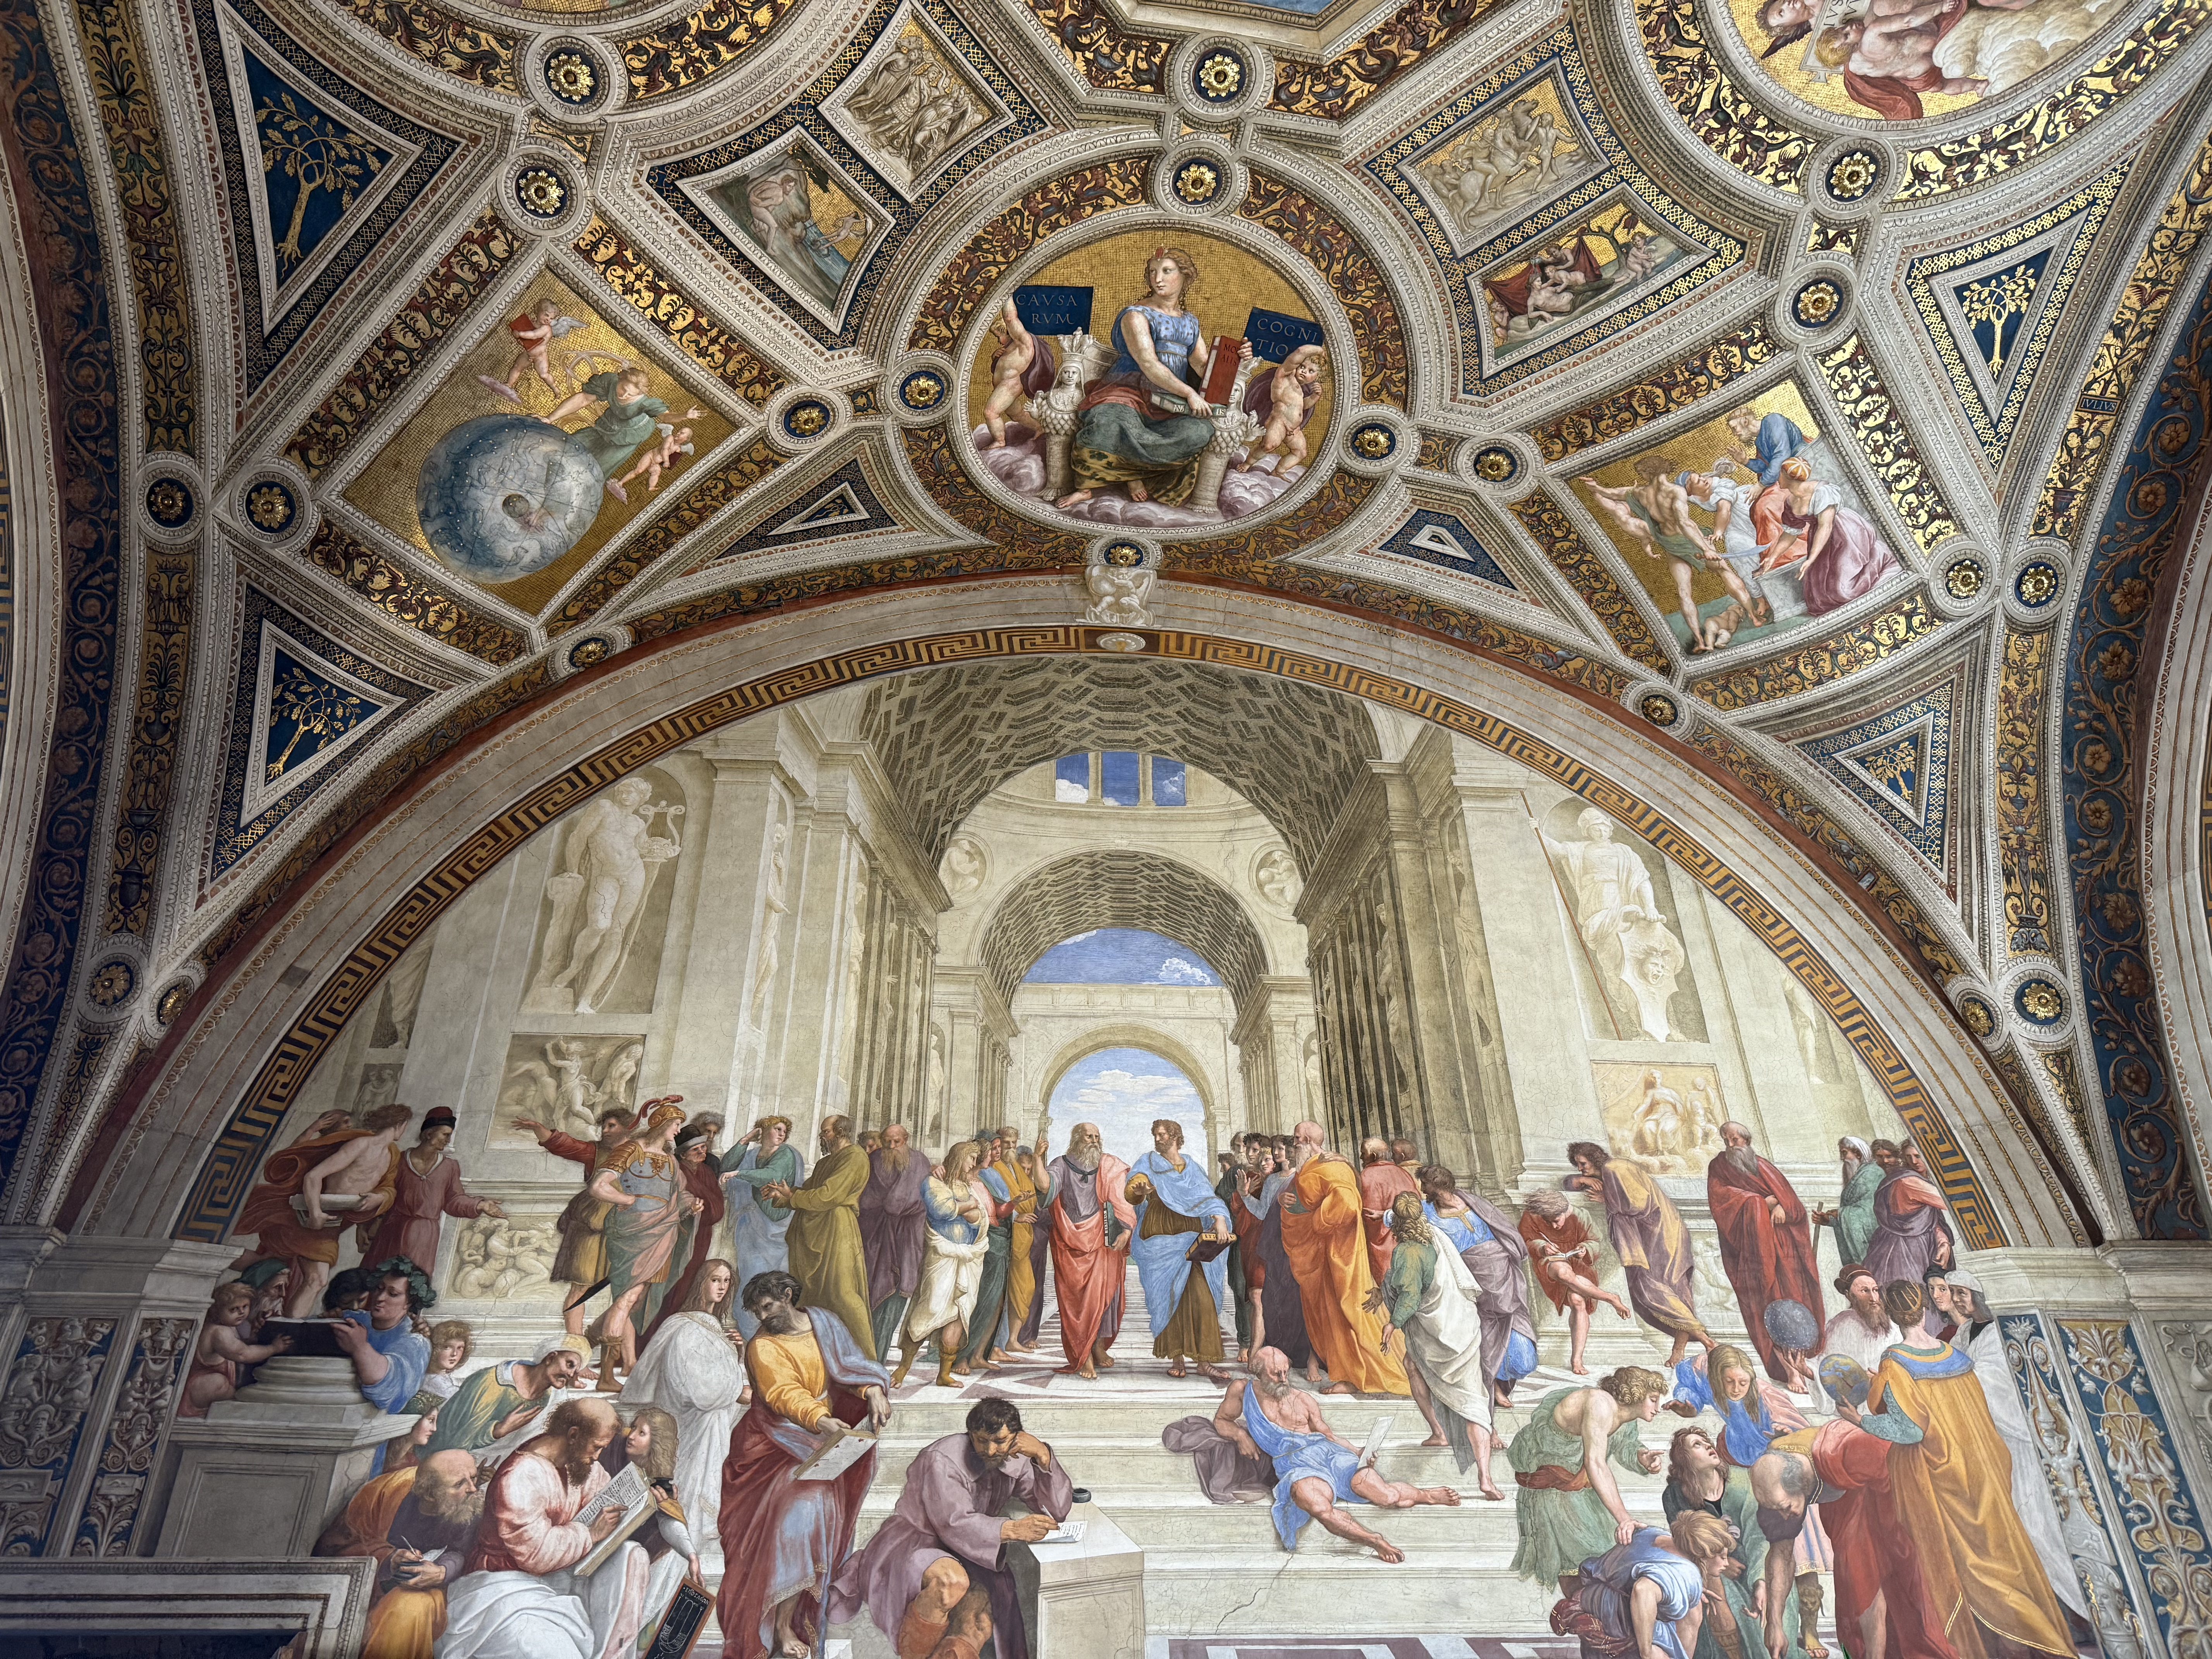
\includegraphics[width=\textwidth]{fig/The_School_of_Athens.jpg}
\end{center}
\end{frame}



\begin{frame}[plain]{Deductive Reasoning}
    \begin{center}
    \includegraphics[width=\textwidth]{fig/black-hole.jpg}
\end{center}
\end{frame}


\begin{frame}[plain]{Inductive Reasoning}
    \begin{center}
    \includegraphics[width=\textwidth]{fig/AI.jpg}
\end{center}
\end{frame}


\begin{frame}{Where is Econometrics Going?}
    \begin{minipage}{0.4\textwidth} % Left side for text
        Covered topics
        \begin{itemize}
            \item Linear models
            \item OLS
            \item Endogeneity
            \item 2SLS, GMM
        \end{itemize}
        
        We will continue...
    \end{minipage}%
    \hfill
    \begin{minipage}{0.6\textwidth} % Right side for image
        \centering
        \includegraphics[width=\textwidth]{fig/30hill.jpg}
    \end{minipage}
\end{frame}



\begin{frame}{Task}
\begin{itemize}

\item Purpose: predict $y$ with $X$
\item Beyond continuous random variables
    \begin{itemize}
        \item Binary
        \item Multi-responses 
        \item Integer
        \item Mixed type: censoring, truncation
        \item Self-selection
    \end{itemize}
\end{itemize}
\end{frame}



\begin{frame}{Likelihood}


\begin{itemize}

    \item Philosophy: The most likely outcome (Abductive reasoning).
    \item Distributional assumption 
\end{itemize}
\begin{center}
    \includegraphics[width=0.45\textwidth]{fig/L(theta).png}
\end{center}
\end{frame}

\begin{frame}{Principles}

\hfill
\includegraphics[width=0.3\textwidth]{fig/Youngronaldfisher.jpeg}
\vspace{-3cm} % Adjust vertical space

\begin{itemize}
\item Hero: Ronald Fisher (1890--1962)

\bigskip

\item General framework
\item Special cases of MLE 
\begin{itemize}
    \item OLS
    \item LIML
\end{itemize}

    
\item Numerical optimization


\end{itemize}

\end{frame}



\begin{frame}{Model Specification}
\begin{itemize}
\item Nature: draws data $Y$ from a parametric model $f$
\item Human: specifies a family of models $g\left(y;\theta\right)$ and a parameter space $\Theta$, which span a \textbf{model space} $G\left(\Theta\right)=\left\{ g\left(y;\theta\right):\theta\in\Theta\right\} $.
\end{itemize}
\begin{center}
    \includegraphics[width=0.8\textwidth]{fig/misspecified.png}
\end{center}
\end{frame}




\begin{frame}{Model and Specification}


\textbf{Parametric model}. The distribution of the data $\mathbf{Y}=\left(Y_{1},...,Y_{N}\right)$
is known up to a finite dimensional parameter.


\bigskip


\begin{itemize}
\item  \textbf{Semiparametric model}: If we know $Y\sim \left(\mu,\sigma^{2}\right)$,
we can estimate $\mu,\sigma^{2}$ by method of moments.
\item \textbf{Parametric model}: If we assume $Y\sim N\left(\mu,\sigma^{2}\right)$,
the model has only two parameters $\mu$ and $\sigma^{2}$. 
\end{itemize}

\end{frame}

\begin{frame}{Likelihood Function}
\begin{itemize}
\item For simplicity, let $\mathbf{Y}=(Y_{1},\ldots,Y_{N})$ be i.i.d.  
\item The \textbf{likelihood} of the sample under a hypothesized value of
$\theta\in\Theta$ is
\[
L\left(\theta;\mathbf{Y}\right)=f\left(\mathbf{Y};\theta\right)=\prod_{i=1}^{N}f\left(Y_{i};\theta \right)
\]

\item Two perspectives:
\begin{itemize}
    \item (Probabilist) $f(\mathbf{Y};\theta)$ is a function of $\mathbf{Y}$ given the parameter $\theta$
    \item (Statistician; reverse engineering) $L(\theta;\mathbf{Y})$ is a function of $\theta$ given the data $\mathbf{Y}$


\end{itemize}

\end{itemize}
\end{frame}



\section{Correct Specification}
\frame{\sectionpage}




\begin{frame}{Log-likelihood}
\begin{itemize}
\item log-likelihood
\[
\ell_{N}\left(\theta\right)
= \log L\left(\theta;\mathbf{Y}\right)
= \sum_{i=1}^{N}\log f\left(Y_{i};\theta\right)
\]
is easier to compute.

\item $\log(\cdot)$ is a monotonically increasing function

\item The MLE estimator
\[
\hat{\theta}=\arg\max_{\theta\in\varTheta}\ell_{N}\left(\theta\right)
\]
\end{itemize}
\end{frame}
%
\begin{frame}{Why Maximization: Deep Justification}
\begin{thm*}
If the model is correctly specified, then $\theta_{0}$ is the maximizer.
\end{thm*}

\begin{itemize}
    \item Kullback-Leibler information criterion (KLIC):
\[
KLIC\left(f,g\right)=\int f\left(z\right)\log\frac{f\left(z\right)}{g\left(z\right)}dz
\]

    \item $KLIC \geq 0$ because 
\begin{align*}
& E\left[\log f\left(Y;\theta_{0}\right)\right]-E\left[\log f\left(Y;\theta\right)\right] \\ 
= & E\left[\log\left(f\left(Y;\theta_{0}\right)/f\left(Y;\theta\right)\right)\right]\\
= & -E\left[\log\left(f\left(Y;\theta\right)/f\left(Y;\theta_{0}\right)\right)\right]\\
\geq & -\log E\left[f\left(Y;\theta\right)/f\left(Y;\theta_{0}\right)\right]=0
\end{align*}
by the Jensen's inequality.

\end{itemize}

\end{frame}


\begin{frame}{KLIC}

    \begin{center}
        \includegraphics[width=\textwidth]{fig/KLIC.png}
    \end{center}

\begin{itemize}
        \item Numerical demon: Normal MLE \url{https://www.kaggle.com/code/frankshi0/normal-mle}
\end{itemize}



\end{frame}


\begin{frame}{Score and Hessian}

\begin{itemize}
\item Score $s_{N}(\theta)=\sum_{i=1}^{N}\frac{\partial}{\partial\theta}\log f(Y_{i};\theta)$ is a function of $\theta$

\item Efficient score $s_{i0}=\frac{\partial}{\partial\theta}\log f\left(Y_{i};\theta_{0}\right)$ is evaluated at the true value $\theta_0$

 

\end{itemize}

\begin{thm*}
If the model is correctly specified, the support of $Y$ does not
depend on $\theta$, and $\theta_{0}$ is in the interior of $\Theta$,
then $E\left[s_{i0}\right]=0$.
\end{thm*}


MLE is equivalent to looking for roots of $s_N(\theta) = 0$.
 

\bigskip

\begin{itemize}

\item Hessian: $H_{N}(\theta)=-\sum_{i=1}^{N}\frac{\partial^{2}}{\partial\theta\partial\theta'}\log f(Y_{i};\theta)$

\item Expected Hessian:
$
H_{0}=-E\left[\frac{\partial^{2}}{\partial\theta\partial\theta'}\log f\left(Y;\theta_{0}\right)\right]
$
\end{itemize}
\end{frame}



\begin{frame}{Score and Hessian: Illustration}
    \begin{center}
        \includegraphics[width=\textwidth]{fig/KLIC.png}
    \end{center}
\end{frame}




\begin{frame}{Information Equality}
\begin{itemize}
\item \textbf{Fisher Information Matrix}: $I_{0}=E[s_{i0}s_{i0}']$ 
\end{itemize}
%
\begin{thm*}
If the model is correctly specified, the support of $Y$ does not
depend on $\theta$, and $\theta_{0}$ is in the interior of $\Theta$,
then $$I_{0}=H_{0}.$$
\end{thm*}
\begin{itemize}

\item Information equality fails when the model is misspecified
\end{itemize}
\end{frame}


\begin{frame}{Cram\'{e}r-Rao Lower Bound}
\begin{thm*}
Suppose the model is correctly specified, the support of $Y$ does
not depend on $\theta$, and $\theta_{0}$ is in the interior of $\Theta$.
If $\widetilde{\theta}$ is unbiased estimator, then $$var(\widetilde{\theta})\geq\left(NI_{0}\right)^{-1}.$$
\end{thm*}

\bigskip

\begin{itemize}
\item More general than OLS's ``BLUE''
\item A lower bound for variance of unbiased estimator
\item When reached, an estimator is called \textbf{Cram\'{e}r-Rao efficient}.
\end{itemize}
\end{frame}
%
\begin{frame}{Example: Normal MLE}
\begin{itemize}
\item Normal distribution $Y_i \sim N(\mu, \sigma^2)$ gives density
$$
f(Y_i | \mu, \sigma^2) = \frac{1}{\sqrt{2\pi \gamma}}
\exp\left(- \frac{(Y_i - \mu)^2 }{2\gamma} \right)
$$
where $\gamma=\sigma^{2}$ to simplify notations and derivatives.

\item The log-likelihood is
\[
\ell_{N}\left(Y;\theta\right)=-\frac{N}{2}\log\gamma-\frac{N}{2}\log2\pi-\frac{1}{2\gamma}\sum_{i=1}^{N}\left(Y_{i}-\mu\right)^{2}
\]
where $\theta = (\mu, \gamma)$. 
\end{itemize}
\end{frame}

% need to compute Fisher info from as the var of score
\begin{frame}{MLE Estimator}

Set the score equal to zero
\[
s_{N}\left(\theta\right)=\left[\begin{array}{c}
\frac{1}{\gamma}\sum_{i=1}^{N}\left(Y_{i}-\mu\right)\\
-\frac{N}{2\gamma}+\frac{1}{2\gamma^{2}}\sum_{i=1}^{N}\left(Y_{i}-\mu\right)^{2}
\end{array}\right]= 0
\]
and we solve the MLE estimator
\[
\hat{\mu} = \frac{1}{N}\sum^{N}_{i=1}Y_{i} = \bar{Y}
\]
\[
\hat{\gamma} = \frac{1}{N}\sum^{N}_{i=1}\left(Y_i-\hat \mu\right)^{2}
=  \frac{1}{N}\sum^{N}_{i=1}\left(Y_i- \bar{Y} \right)^{2}
\]

\end{frame}

\begin{frame}{Lower Bound}

\begin{itemize}

\item The Hessian
\[
H_{N}\left( \theta \right)=\left[\begin{array}{cc}
\frac{N}{\gamma} & \frac{1}{\gamma^{2}}\sum_{i=1}^{N}\left(Y_{i}-\mu\right)\\
\star & -\frac{N}{2\gamma^{2}}+\frac{1}{\gamma^{3}}\sum_{i=1}^{N}\left(Y_{i}-\mu\right)^{2}
\end{array}\right]
\]

\item Expectation:
$
E\left[H_{N}\left(\theta_0 \right)\right]=\left[\begin{array}{cc}
\frac{N}{\gamma} & 0\\
0 & \frac{N}{2\gamma^{2}}
\end{array}\right] = N \times H_0
$


\item Take inverse:
$
\left[\begin{array}{cc}
\frac{\gamma}{N} & 0\\
0 & \frac{ 2\gamma^{2}}{N}
\end{array}\right]
$

\item Information equality can be verified.

\end{itemize}
\end{frame}

%
\begin{frame}{MLE for the Mean}
\begin{itemize}
    \item The sample mean
\[
var\left(\frac{1}{N}\sum_{i=1}^{N}Y_{i}\right)=\frac{\sigma^{2}}{N}
\]
reaches the  Cram\'{e}r-Rao lower bound
\end{itemize}
\end{frame}
%
\begin{frame}{MLE for the Variance}
\begin{itemize}
\item $E\left(S_{N}^{2}\right)=\sigma^{2}$ is unbiased, where
\[
s_{N}^{2}=\frac{1}{N-1}\sum_{i=1}^{N}\left(Y_{i}-\bar{Y}\right)^{2}=\frac{1}{N-1}Y'\left(I-\frac{1}{N}1_{N}1_{N}'\right)Y
\]
\item It follows
$s_{N}^{2}=\frac{\sigma^{2} }{N-1} \cdot \chi^{2}\left(N-1\right)$ because

\[
\left(N-1\right)\frac{s_{N}^{2}}{\sigma^{2}}=\left(\frac{Y}{\sigma}\right)'\left(I-\frac{1}{N}1_{N}1_{N}'\right)\left(\frac{Y}{\sigma}\right)\sim\chi^{2}\left(N-1\right).
\]
\item As a result, 
\[
var\left(s_{N}^{2}\right)=\frac{\sigma^{4}}{\left(N-1\right)^{2}} \cdot 2\left(N-1\right)=\frac{2\sigma^{4}}{N-1}>\frac{2\sigma^{4}}{N}
\]
Is not Cram\'{e}r-Rao efficient
\end{itemize}
\end{frame}
%

\begin{frame}{Return to Normal Regression}

\begin{itemize}
    \item The normal regression models is 
$$Y_{i}=X_{i}'\beta+\varepsilon_{i}$$
     \item Under the assumption $\varepsilon_{i} \mid X_{i}\sim N \left(0,\gamma \right),$ the conditional distribution is 
     $$Y_{i} \mid X_{i} \sim N \left( X_{i}'\beta,\gamma\right).$$

    \item Parameter $\theta = (\beta, \gamma)$
    \item The joint likelihood $$f(Y_i , X_i) = f(Y_i | X_i) f(X_i),$$ where the specification of $f(X_i)$ is irrelevant to $\theta$.
\end{itemize}
\end{frame}


     
\begin{frame}{Conditional Log-Likelihood}
\begin{itemize}
     \item  The \textbf{conditional log-likelihood} of the sample is $$\ell_N (\theta) 
     = -\frac{N}{2}\log\gamma -\frac{N}{2}\log 2\pi - \frac{1}{2\gamma} \sum_{i=1}^{N} \left(Y_{i}-X_{i}^{\prime}\beta\right)^{2},
     $$ where the distribution of $X_i$ is unspecified.

     \item The MLE estimator $$\hat{\beta} = (X'X)^{-1} X'Y$$
     $$\hat{\sigma}^2 = \frac{1}{N} \sum_{i=1}^N \hat{\varepsilon}_i^2 $$
     where $\hat{\varepsilon}_i = Y_i - X_i' \hat{\beta}$.
\end{itemize}
\end{frame}

\begin{frame}{Asymptotic Normality}
\begin{itemize}

\item Under regularity conditions, $\hat{\theta}\stackrel{p}{\to}\theta_{0}$, and
\[
\sqrt{N}\left(\hat{\theta}-\theta_{0}\right)\stackrel{d}{\to}N\left(0,H_{0}^{-1}I_{0}H_{0}^{-1}\right)
\]
\item When the information equality holds, we have 
\[
\sqrt{N}\left(\hat{\theta}-\theta_{0}\right)\stackrel{d}{\to}N\left(0,I_{0}^{-1}\right),
\]
or equivalently
\[
\hat{\theta}-\theta_{0} \stackrel{a}{\sim}N\left(0,\frac{I_{0}^{-1}}{N}\right),
\]
\item The variance $(N I_0)^{-1}$ is efficient!

\end{itemize}


\end{frame}




\section{Mispecification}
\frame{\sectionpage}



\begin{frame}[plain]{KLIC for Misspecified Models}

\begin{center}
    \includegraphics[width=0.7\textwidth]{fig/misspecified.png}
\end{center}
\begin{itemize}
\item If $f\notin G\left(\Theta\right)$, the model is  misspecified. 
\begin{align*}
KLIC\left(f,g\left(y;\theta\right)\right) & =\int f\left(y\right)\log f\left(y\right)dy-\int f\left(y\right)\log g\left(y;\theta\right)dy\\
 & =E\left[\log f\left(y\right)\right]-E\left[\log g\left(y;\theta\right)\right] > 0
\end{align*}

\end{itemize}
\end{frame}




\begin{frame}{Misspecified Model}
\begin{itemize}

\item Misspecified: $\min_{\theta\in\Theta}KLIC\left(f,g\left(y;\theta\right)\right)>0$
\item MLE is still meaningful

\item Pseudo-true parameter:
\[
\theta^{*}=\arg\max_{\theta\in\Theta} E [\ell\left(\theta\right)]
\]
the minimizer of $KLIC\left(f,g\left(y;\theta\right)\right)$ in the
parameter space $\Theta$
\item Under standard assumption, the MLE estimator $\widehat{\theta}\stackrel{p}{\to}\theta^{*}$ and 
\[
\sqrt{N}\left(\hat{\theta}-\theta^{*}\right)\stackrel{d}{\to}N\left(0,H_{*}^{-1}I_{*}H_{*}^{-1}\right)
\]
%
\end{itemize}
\end{frame}


\begin{frame}{Three Tests}

A linear hypothesis: $R \theta_0 = q$.
    \bigskip
    
    \begin{itemize}
        \item Wald test: unconstrained estimation, $\ell_N (\hat{\theta}) $ 
        \item Lagrange multiplier test: constrained estimation under the null, $\ell_N (\tilde{\theta})$
        \item Likelihood ratio test: $ \ell_N (\hat{\theta}) - \ell_N (\tilde{\theta})$
    \end{itemize}

\bigskip

Also works for nonlinear hypothesis.

\bigskip

Are specification tests important?

\end{frame}

\begin{frame}{Summary}

\begin{itemize}
    \item Parametric models
    \item Specification of distribution family
    \item MLE
    \item Score, Hessian, information matrix
    \item Misspecification
\end{itemize}
    
\end{frame}



% \begin{frame}{My Related Research}
%     \begin{itemize}
%         \item Ming Li, Zhentao Shi, and Yapeng Zheng (2024) ``Estimation and Inference in Dyadic Network Formation Models with Nontransferable Utilities'', \emph{working paper}. \url{https://arxiv.org/abs/2410.23852}
%         \item Jinyuan Chang, Zhentao Shi and Jia Zhang (2023): ``Culling the Herd of Moments with Penalized Empirical Likelihood,'' \emph{Journal of Business \& Economic Statistics}, 41(3), 791-805. \url{https://doi.org/10.1080/07350015.2022.2071903}
%         \item Zhentao Shi (2016): ``Econometric Estimation with High-Dimensional Moment Equalities,'' \emph{Journal of Econometrics}, 195, 104-119. \url{https://doi.org/10.1016/j.jeconom.2016.07.004}
%     \end{itemize}
    
\end{frame}

\end{document}


% to continue with limited dependent variables